\documentclass[journal]{IEEEtran}
\usepackage[T1]{fontenc}
\usepackage[utf8]{inputenc}
\usepackage{amsmath,amssymb}
\interdisplaylinepenalty=2500
\usepackage{graphicx}
\usepackage{booktabs}
\usepackage{multirow}
\usepackage{array}
\usepackage{tabularx}
\usepackage{url}
\usepackage{xcolor}
\usepackage{cite}
\usepackage{longtable}
\usepackage{xurl}
\usepackage{hyperref}

\hypersetup{
  pdftitle={Composing an Authority Layer with a Sandbox Runtime: BULL on NVIDIA OpenShell},
  pdfauthor={Luis Minier},
  pdfsubject={Empirical qualification of BULL execution governance composed with NVIDIA OpenShell v0.1.2 through its supervisor-middleware and gateway-interceptor extension points},
  pdfkeywords={AI-agent security, execution governance, sandbox runtime, OpenShell, supervisor middleware, gateway interceptor, provenance, fail-closed, OCSF, audit integrity},
  colorlinks=false,
  pdfborder={0 0 0}
}

\newcolumntype{Y}{>{\raggedright\arraybackslash}X}
\newcommand{\bull}{\textsc{BULL}}
\newcommand{\openshell}{OpenShell}
\newcommand{\expshort}{\texttt{56faa30}}
\newcommand{\baseshort}{\texttt{6682adb}}
\newcommand{\osshort}{\texttt{6648bd0}}
\newcommand{\medGetA}{8.98}
\newcommand{\medGetB}{17.07}
\newcommand{\deltaGet}{8.08}
\newcommand{\ciLoGet}{7.12}
\newcommand{\ciHiGet}{8.86}
\newcommand{\pNineGetA}{16.92}
\newcommand{\pNineGetB}{26.03}
\newcommand{\nLatGet}{200}
\newcommand{\driftFirstGetB}{14.89}
\newcommand{\driftLastGetB}{17.67}
\newcommand{\driftFirstGetA}{9.07}
\newcommand{\driftLastGetA}{9.68}
\newcommand{\medPostA}{9.85}
\newcommand{\medPostB}{20.83}
\newcommand{\deltaPost}{10.98}
\newcommand{\ciLoPost}{10.16}
\newcommand{\ciHiPost}{11.72}
\newcommand{\pNinePostA}{21.19}
\newcommand{\pNinePostB}{34.20}
\newcommand{\nLatPost}{200}
\newcommand{\driftFirstPostB}{19.49}
\newcommand{\driftLastPostB}{25.13}
\newcommand{\driftFirstPostA}{10.33}
\newcommand{\driftLastPostA}{9.20}
\newcommand{\createMeanA}{914}
\newcommand{\createMeanB}{986}
\newcommand{\createDelta}{71}
\newcommand{\createN}{6}
\newcommand{\gapMedian}{5}
\newcommand{\gapMin}{1}
\newcommand{\gapMax}{7}
\newcommand{\gapN}{10}
\newcommand{\corrDecisions}{9}
\newcommand{\corrMatched}{9}
\newcommand{\corrConsistent}{9}
\newcommand{\corrUnexplained}{0}
\newcommand{\corrOrphans}{1}
\newcommand{\ledgerRecordsCTen}{19}
\newcommand{\ledgerRecordsTotal}{431}
\newcommand{\ocsfEventsB}{21}
\newcommand{\ocsfEventsA}{8}
\newcommand{\receiptsA}{7}
\newcommand{\receiptsB}{5}
\newcommand{\passA}{12}
\newcommand{\totalA}{12}
\newcommand{\passB}{14}
\newcommand{\totalB}{14}
\newcommand{\passAll}{26}
\newcommand{\totalAll}{26}
\newcommand{\osVersion}{v0.1.2}
\newcommand{\hostKernel}{6.18.44-fc-v37}
\newcommand{\dockerVersion}{Docker version 29.3.1, build c2be9cc}


\begin{document}

\title{Composing an Authority Layer with a Sandbox Runtime: \bull{} on NVIDIA \openshell}

\author{Luis~Minier%
\thanks{Luis Minier is an independent researcher at Anharmoniclabs. Technical report, version 0.1, September 28, 2026. Author-review manuscript; not peer-reviewed. Experiment branch \texttt{experiment/bull-openshell-20260928}; tested \bull{} source commit \expshort.}}

\maketitle

\begin{abstract}
A sandbox runtime decides \emph{where} an agent's code may reach; an authority layer decides \emph{whether a specific action, given where its inputs came from, is authorized and by whom}. This report tests whether the two can be composed without the composition itself opening a bypass. \bull{}, an execution-governance runtime with signed grants, provenance tracking, single-use human approvals, and a hash-chained ledger, was implemented as an NVIDIA \openshell{} supervisor middleware and gateway interceptor and evaluated against a live \openshell{} \osVersion{} gateway built from source (commit \osshort) on the Docker compute driver. The invariant under test is $\mathrm{Effect}(r) \Rightarrow \mathrm{BULL}(r) \wedge \mathrm{OpenShell}(r)$, with absence of \bull{} implying no effect. A ten-case proof suite plus two added cases was run in two phases---\openshell{} alone and \openshell{} with \bull{} registered fail-closed---and every outcome was judged at the destination service, not from client output. In the final run \passAll{} of \totalAll{} checks behaved as specified; with \bull{}, \passB{} of \totalB{} properties held, including approval-gated exfiltration after untrusted input, refusal of unapproved policy widening and credential attachment, fail-closed behavior when \bull{} was killed, and a join of \corrConsistent{} of \corrDecisions{} \bull{} decisions to \openshell{}'s OCSF telemetry with zero effects lacking a \bull{} allow. Composition added a median \deltaGet{}\,ms per GET (95\% CI [\ciLoGet, \ciHiGet]) and \deltaPost{}\,ms per POST ([\ciLoPost, \ciHiPost]), $n=\nLatGet$ each. The experiment also surfaced findings about both systems: \openshell{}'s L7 rules default to an audit mode that forwards violations, its middleware requests misreport scheme and omit the originating process, and \bull{}'s ledger append is $O(n)$ in ledger length. Six integration defects in \bull{} were found only against the live gateway and fixed. These are project-authored results from a single host, not independent certification.
\end{abstract}

\begin{IEEEkeywords}
AI-agent security, execution governance, sandbox runtime, OpenShell, supervisor middleware, gateway interceptor, provenance, fail-closed, OCSF, audit integrity.
\end{IEEEkeywords}

%%% ------------------------------------------------------------------
\section{Introduction}
%%% ------------------------------------------------------------------
\IEEEPARstart{A}{gent} sandboxes and agent authority layers answer different questions. NVIDIA \openshell{} runs each agent in a sandbox whose declarative network and filesystem policy, enforced by a per-sandbox supervisor, bounds the hosts, ports, methods, paths, and binaries the workload can use, and it emits OCSF security telemetry for what it allows and denies~\cite{OS_Repo,OS_Logging}. It does not know that the text an agent just read came from an attacker, and anyone able to call its configuration API can widen a policy. \bull{} treats agent output as a proposal and binds execution to host-owned authority, provenance, and approvals~\cite{BULL_Report}; but a decision layer binds only the traffic that passes through it.

\openshell{} exposes two extension points that make composition possible without modifying either system: a \emph{supervisor middleware} called for each proxied HTTP request after \openshell{}'s own policy and before credential injection, and a \emph{gateway interceptor} called on control-plane RPCs, able to patch a proposed operation or refuse it~\cite{OS_MiddlewareDoc,OS_InterceptorDoc}. This report asks three questions. \textbf{RQ1:} Can \bull{} be composed through these extension points as a narrowing-only layer, such that an effect requires both systems' consent? \textbf{RQ2:} Does the composition fail closed when \bull{} is absent, and can the two systems' records be joined into one trail? \textbf{RQ3:} What does the composition cost, and what does exercising it reveal about either component?

\subsection{Scope and Evidence Discipline}
This report separates four evidence classes: (1) upstream \openshell{} source and documentation at tag \texttt{v0.1.2}; (2) \bull{} source on the experiment branch; (3) measurements from one automated two-phase run on one host, whose raw files are hashed in Supplement~S6; and (4) limitations and experiments not performed. All tables, figures, and in-text numbers are generated from the evidence files by the build script; none are transcribed by hand. A passing case demonstrates the stated behavior for this configuration; it is not proof against unknown attacks.

%%% ------------------------------------------------------------------
\section{Threat Model and Composition Contract}
%%% ------------------------------------------------------------------
\subsection{Adversaries and Assets}
The untrusted side is the sandboxed workload and everything it reads: model output, fetched content, and processes it starts. Three adversary behaviors are exercised: a workload that attempts an effect it was not granted; a workload steered by untrusted content toward exfiltration through an allowed endpoint; and a caller of the \openshell{} API who attempts to widen a sandbox's authority or attach a credential. Protected assets are effects at destination services, provider credentials, and the integrity of the combined audit record.

\subsection{Trusted Computing Base}
Both systems are trusted: the \openshell{} gateway, supervisor, and sandbox runtime; the Docker daemon and Linux kernel; the \bull{} authority process, its signing key, and its ledger; and the operator who approves escalations. A malicious host administrator and a compromised kernel or container runtime are out of scope. In this experiment the middleware transport was not authenticated (Section~\ref{sec:limits}); that is a deviation from a production trust configuration, not an assumption about it.

\subsection{Contract}
Let $r$ be a request from sandbox $s$. Let $\mathrm{OS}(r)$ denote \openshell{}'s network and L7 policy decision and $\mathrm{B}(r)$ \bull{}'s decision. The composition is intended to satisfy
\begin{align*}
\mathrm{Effect}(r) \implies{} & \mathrm{OS}(r) \land \mathrm{B}(r), \\
\neg\mathrm{Available}(\bull) \implies{} & \neg\mathrm{Effect}(r) \land \neg\mathrm{Admit}(s'), \\
\mathrm{Policy}_{t+1}(s) \supsetneq \mathrm{Policy}_t(s) \implies{} & \mathrm{Approved}(\Delta), \\
\mathrm{Effect}(r) \implies{} & \exists\, \ell \in \mathrm{Ledger}: \ell \sim r,
\end{align*}
where $s'$ is a sandbox being created, $\Delta$ the added endpoints, and $\ell \sim r$ a ledger record joinable to $r$'s OCSF events. $\mathrm{B}$ is \emph{narrowing only}: the middleware can return allow or deny, never widen \openshell{}'s decision, and the interceptor can only attach \bull{}'s middleware or refuse.

%%% ------------------------------------------------------------------
\section{Design}
%%% ------------------------------------------------------------------
\subsection{Data Plane: Supervisor Middleware}
\bull{} registers one binding: HTTP request, phase \texttt{PRE\_CREDENTIALS}, 256\,KiB payload ceiling~\cite{OS_MiddlewareProto}. For each request, \texttt{GET}/\texttt{HEAD}/\texttt{OPTIONS} map to capability \texttt{network.outbound} and other methods to \texttt{network.post}; the sandbox's signed grant must contain the capability. A sandbox's provenance becomes \texttt{internet} once it performs an allowed read from a \texttt{host:port} not listed as trusted; afterwards \bull{}'s deterministic policy escalates any \texttt{network.post}. An escalation creates a pending approval bound to method, URL, and body hash; an operator's approval admits that exact request once. Every decision is appended to \bull{}'s hash-chained ledger. Taint and approvals persist across restarts.

\subsection{Control Plane: Gateway Interceptor}
\bull{} governs \texttt{CreateSandbox} and \texttt{UpdateConfig} in the \texttt{modify\_operation} and \texttt{validate} phases, and \texttt{AttachSandboxProvider}, \texttt{ApproveDraftChunk}, \texttt{ApproveAllDraftChunks}, and \texttt{EditDraftChunk} in \texttt{validate}~\cite{OS_InterceptorProto}. \texttt{modify\_operation} returns RFC~6902 patches~\cite{RFC6902} that attach \bull{}'s middleware with \texttt{onError: fail\_closed} to every host of a new or replacement policy. \texttt{validate} refuses: sandboxes not fully mediated; hosts outside the signed ceiling; L7 rules not in \texttt{enforce} mode; any new \texttt{host:port} or new L7 rule set without a matching single-use approval; all draft-policy approvals without \bull{} approval; global policy changes; and provider attachment for sandboxes lacking a \texttt{credential.read} grant. Both extensions are registered with \texttt{failure\_policy = fail\_closed}.

\subsection{Grants and Audit Join}
Per-sandbox grants (capabilities, trusted \texttt{host:port} sources, and a global host ceiling) are embedded in \bull{}'s HMAC-signed policy bundle. For the audit join, \openshell{}'s supervisor pushes OCSF events to the gateway, which serves them in shorthand~\cite{OS_Logging}. A correlator matches each \bull{} ledger decision to the \openshell{} L7 and middleware events of the same sandbox, method, and target within a time window, and assigns destination receipts only to decisions \bull{} allowed; any receipt left unassigned is an effect \bull{} never allowed.

%%% ------------------------------------------------------------------
\section{Method}
%%% ------------------------------------------------------------------
\subsection{Environment and Deviations}
Table~\ref{tab:env} records the environment. The session's network policy blocked the official installer and image registries, so all binaries and images were built locally from the upstream source and Dockerfiles, with two deviations: the supervisor image used \texttt{distroless/cc-debian13} instead of the pinned \texttt{base-nossl-debian13}, because a locally linked supervisor requires \texttt{libgcc\_s}; and \texttt{host.openshell.internal} was mapped on the host to the Docker bridge (172.17.0.1) so that the host-resident gateway reaches the middleware at the address the supervisors use. Policies list \texttt{allowed\_ips: [172.17.0.1/32]} because \openshell{}'s SSRF guard otherwise refuses private destinations~\cite{OS_Logging}.

\begin{table}[!t]
\caption{Experimental Environment}
\label{tab:env}
\centering
\small
\begin{tabularx}{\columnwidth}{lY}
\toprule
\textbf{Item} & \textbf{Value} \\
\midrule
\openshell{} & \osVersion{}, tag \texttt{v0.1.2}, commit \osshort{}; gateway, CLI, supervisor glibc; sandbox runtime static musl; Rust 1.95.0 \\
Compute driver & \dockerVersion{}, pull policy \texttt{never} \\
Host & Linux \hostKernel{}, 4 vCPU, 15\,GiB, shared cloud container \\
Sandbox image & \texttt{ubuntu:24.04} + curl, python3; uid 1500 \\
\bull{} & commit \expshort{}; Python 3.11; grpcio 1.84; protobuf 7.36 \\
Transport & middleware: plaintext gRPC on bridge; interceptor: Unix socket \\
\bottomrule
\end{tabularx}
\end{table}

\subsection{Topology and Grants}
Three host services record every request that reaches them: \emph{docs} (trusted by \bull{}), \emph{news} (untrusted; returns a prompt-injection string), and \emph{api} (the effect target). \openshell{}'s policy allows \texttt{GET /**} on docs and news and \texttt{POST /v1/**} on api, each with \texttt{enforcement: enforce} and binary \texttt{/usr/bin/curl}. \bull{} grants sandbox \texttt{coder} outbound and post, \texttt{reader} outbound only, and \texttt{bench} outbound and post; all trust only docs; the ceiling is \texttt{host.openshell.internal}.

\subsection{Phases, Judging, and Measurement}
Phase~A runs \openshell{} alone; Phase~B runs the same requests with both \bull{} extensions registered. A case passes on destination evidence: a request is ``blocked'' only if the destination never received it. Phase~A rows for \bull{}-specific properties record what \openshell{} alone does; their ``as expected'' status means the observation was made, not that the property holds. Latency is \texttt{curl}'s \texttt{time\_total} for \nLatGet{} trusted GETs and \nLatPost{} allowed POSTs in one in-sandbox loop, excluding exec overhead; admission time is \texttt{sandbox create --detach} wall time over \createN{} creations and measures admission including interceptor round trips, not boot to Ready. The harness (\texttt{tools/openshell\_experiment.py}) is fully automated.

%%% ------------------------------------------------------------------
\section{Results}
%%% ------------------------------------------------------------------
\subsection{Proof Suite}
Table~\ref{tab:cases} and Fig.~\ref{fig:outcomes} give the outcomes. In Phase~A, \passA{} of \totalA{} observations were as expected; in Phase~B, \passB{} of \totalB{} properties held (both counts include two setup rows). The complete observed output of every case is reproduced in Supplement~S1.

\begin{table*}[!t]
\caption{Proof-Suite Outcomes, Judged at the Destination}
\label{tab:cases}
\centering
\scriptsize
\begin{tabularx}{\textwidth}{l>{\raggedright\arraybackslash}p{3.6cm}YYl}
\toprule
\textbf{Case} & \textbf{Property} & \textbf{A: \openshell{} only} & \textbf{B: \openshell{} + \bull{}} & \textbf{B} \\
\midrule
C1 & BULL ALLOW $\wedge$ OpenShell ALLOW executes & HTTP 200; effect reached upstream & HTTP 200; effect reached upstream & \textbf{held} \\
C2 & BULL DENY $\wedge$ OpenShell ALLOW is blocked & HTTP 200; effect reached upstream & HTTP 403; no effect & \textbf{held} \\
C3 & BULL ALLOW $\wedge$ OpenShell DENY is blocked & HTTP 403; no effect & HTTP 403; no effect & \textbf{held} \\
C3b & L7 rules left at default (audit) enforcement & created; out-of-rule POST reached upstream & creation refused (enforcement not enforce) & \textbf{held} \\
C4 & ESCALATE: no effect before approval, one after & HTTP 200; effect reached upstream & HTTP 403 $\rightarrow$ approve $\rightarrow$ 200 $\rightarrow$ reuse 403; upstream count 1 & \textbf{held} \\
C5 & Unauthorized policy widening rejected & applied (policy v3 loaded) & refused: approval required for 'host.openshell.internal:9' & \textbf{held} \\
C5b & Host outside signed ceiling rejected & --- & refused: outside signed ceiling & \textbf{held} \\
C6 & Provider credential never readable & canary not in sandbox env; attach pending supervisor & attach refused; canary not in env & \textbf{held} \\
C7 & Internet-derived content $\rightarrow$ POST & effect reached upstream & HTTP 403; no effect & \textbf{held} \\
C8 & Native bypass contained & \texttt{-{}-noproxy} POST reached (OCSF: l7); other binary, raw socket, UDP DNS failed & \texttt{-{}-noproxy} POST blocked (OCSF: l7+middleware); other binary, raw socket, UDP DNS failed & \textbf{held} \\
C9 & BULL unavailable $\Rightarrow$ fail closed & --- & POST HTTP 403, no effect; create refused; after restart GET 200 & \textbf{held} \\
C10 & One correlatable audit trail & 8 OCSF L7 events; no authority record & 9/9 decisions consistent; 0 effects w/o allow; ledger valid & \textbf{held} \\
\bottomrule

\end{tabularx}
\end{table*}

\begin{figure*}[!t]
\centering
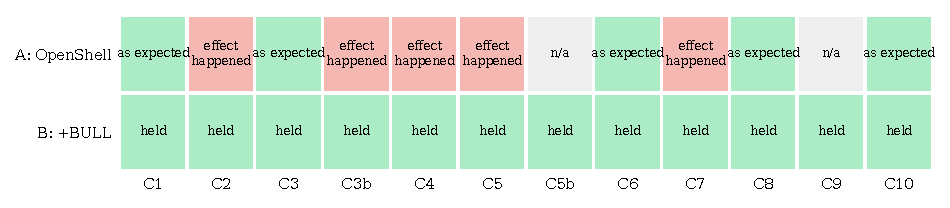
\includegraphics[width=\textwidth]{figs/outcomes.pdf}
\caption{Outcome matrix. Red cells in row~A mark effects that \openshell{} alone permitted and the composed system blocked; ``n/a'' marks cases that exist only with \bull{}.}
\label{fig:outcomes}
\end{figure*}

Three results carry most of the weight. First, in C2, C4, and C7, \openshell{}'s own L7 engine allowed every request (Table~\ref{tab:corr}), so the blocked effects in Phase~B are attributable to \bull{} alone: without an authority layer, a sandbox that read attacker-controlled content posted to the allowed API (C7-A). Second, C4 shows exactly-once semantics: a pending escalation produced no effect, an approval admitted one request, and reusing the approval was refused, leaving exactly one upstream record. Third, C9 killed the \bull{} process: the next POST was denied by \openshell{} with \texttt{middleware\_failed: external\_service\_error} and never reached the destination, sandbox creation was refused, and after restart a trusted read succeeded with persisted taint and approvals intact.

\subsection{Unified Audit Trail}
Table~\ref{tab:corr} lists every Phase~B \bull{} decision joined to \openshell{}'s telemetry and to the destination. All \corrMatched{} of \corrDecisions{} decisions matched an \openshell{} middleware event, \corrConsistent{} were consistent in decision and effect, and \corrUnexplained{} destination receipts lacked a \bull{} allow. The single \openshell{} middleware event with no \bull{} decision (\corrOrphans{}) is the C9 fail-closed denial issued while \bull{} was down. The ledger verified intact at \ledgerRecordsCTen{} records at the time of C10. \openshell{} carries \bull{}'s reason code into its own denial telemetry (e.g., \texttt{middleware\_denied:\allowbreak bull-governance:\allowbreak bull\_approval\_required}), so an OCSF-only consumer still sees why \bull{} refused.

\begin{table*}[!t]
\caption{Phase B Audit Join: \bull{} Ledger $\times$ \openshell{} OCSF $\times$ Destination (* = approval bound)}
\label{tab:corr}
\centering
\scriptsize
\begin{tabular}{rllllllll}
\toprule
\# & \textbf{Sandbox} & \textbf{Method} & \textbf{Target} & \textbf{\bull{}} & \textbf{OS L7} & \textbf{OS middleware} & \textbf{Effect} & \textbf{Consistent} \\
\midrule
1 & coder & GET & :40959/guide & ALLOW & ALLOWED & ALLOWED & yes & yes \\
2 & coder & POST & :35911/v1/records & ALLOW & ALLOWED & ALLOWED & yes & yes \\
3 & reader & POST & :35911/v1/records & DENY & ALLOWED & DENIED & no & yes \\
4 & coder & GET & :46731/article & ALLOW & ALLOWED & ALLOWED & yes & yes \\
5 & coder & POST & :35911/v1/records & ESCALATE* & ALLOWED & DENIED & no & yes \\
6 & coder & POST & :35911/v1/records & ESCALATE* & ALLOWED & ALLOWED & yes & yes \\
7 & coder & POST & :35911/v1/records & ESCALATE* & ALLOWED & DENIED & no & yes \\
8 & coder & POST & :35911/v1/x & ESCALATE* & ALLOWED & DENIED & no & yes \\
9 & coder & GET & :40959/after-restart & ALLOW & ALLOWED & ALLOWED & yes & yes \\
\bottomrule

\end{tabular}
\end{table*}

\subsection{Latency}
Table~\ref{tab:latency} and Figs.~\ref{fig:dist}--\ref{fig:create} summarize performance. Composition increased median request latency from \medGetA{} to \medGetB{}\,ms for GET and from \medPostA{} to \medPostB{}\,ms for POST. Table~\ref{tab:stats} gives bootstrap confidence intervals (10\,000 resamples, fixed seed) and two-sided Mann--Whitney tests. From OCSF timestamps, \openshell{}'s L7 event preceded \bull{}'s verdict by a median of \gapMedian{}\,ms (range \gapMin--\gapMax{}\,ms, $n=\gapN$, 1\,ms resolution); this interval contains the plaintext gRPC round trip, the Python decision, and a synchronous ledger append. Mean admission time rose by \createDelta{}\,ms ($n=\createN$), which is within run-to-run spread.

\begin{table}[!t]
\caption{Latency Summary (Requests in ms; Creation in ms)}
\label{tab:latency}
\centering
\scriptsize
\setlength{\tabcolsep}{2.6pt}
\begin{tabular}{llrrrrrrrr}
\toprule
\textbf{Metric} & \textbf{Ph.} & $n$ & \textbf{Mean} & \textbf{Med.} & \textbf{p95} & \textbf{p99} & \textbf{Min} & \textbf{Max} & $\sigma$ \\
\midrule
GET & A & 200 & 10.23 & 8.98 & 16.92 & 23.38 & 6.36 & 31.20 & 3.49 \\
GET & B & 200 & 17.88 & 17.07 & 26.03 & 30.69 & 11.43 & 43.46 & 4.34 \\
POST & A & 200 & 11.46 & 9.85 & 21.19 & 27.43 & 6.64 & 33.86 & 4.60 \\
POST & B & 200 & 22.65 & 20.83 & 34.20 & 40.64 & 14.42 & 65.33 & 6.60 \\
Create & A & 6 & 914 & 924 & 1004 & 1022 & 811 & 1026 & 67 \\
Create & B & 6 & 986 & 996 & 1046 & 1056 & 908 & 1058 & 48 \\
\bottomrule

\end{tabular}
\end{table}

\begin{table}[!t]
\caption{Overhead (B $-$ A): Median Difference, 95\% Bootstrap CI, Mann--Whitney U}
\label{tab:stats}
\centering
\scriptsize
\setlength{\tabcolsep}{3pt}
\begin{tabular}{lrrrrrr}
\toprule
\textbf{Metric} & $\Delta$\textbf{med} & \textbf{95\% CI} & $U$ & $z$ & $p$ & $|r|$ \\
\midrule
GET & +8.08 & [+7.12, +8.86] & 2525 & -15.11 & $<10^{-15}$ & 0.874 \\
POST & +10.98 & [+10.16, +11.72] & 2470 & -15.16 & $<10^{-15}$ & 0.877 \\
\bottomrule

\end{tabular}
\end{table}

\begin{figure}[!t]
\centering
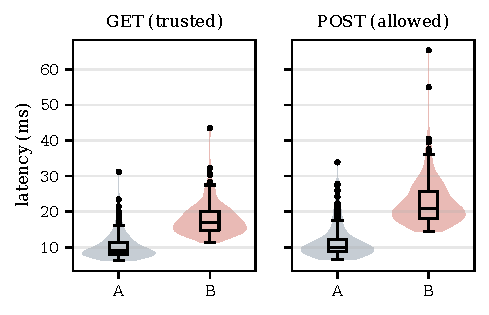
\includegraphics[width=\columnwidth]{figs/distributions.pdf}
\caption{Per-request latency distributions, $n=\nLatGet$ per cell.}
\label{fig:dist}
\end{figure}

\begin{figure}[!t]
\centering
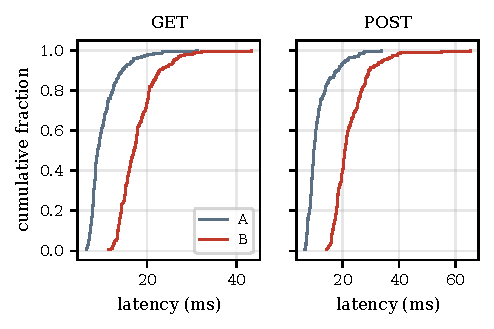
\includegraphics[width=\columnwidth]{figs/ecdf.pdf}
\caption{Empirical CDFs of request latency for Phases A and B.}
\label{fig:ecdf}
\end{figure}

\begin{figure*}[!t]
\centering
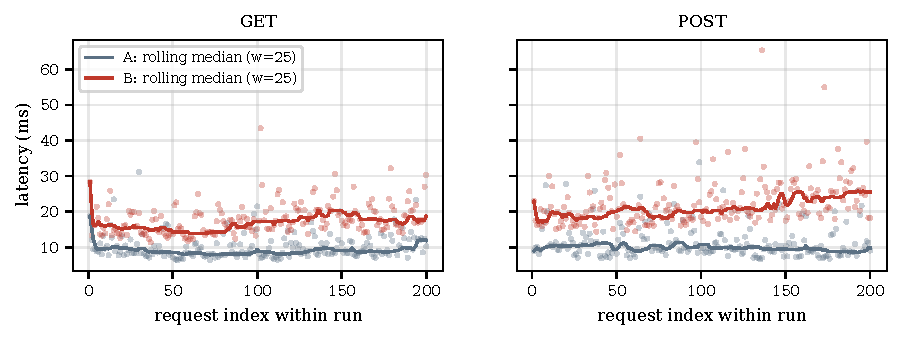
\includegraphics[width=\textwidth]{figs/drift.pdf}
\caption{Latency by request index. Phase~B's rolling median rises through the run while Phase~A's stays flat (Table~\ref{tab:drift}).}
\label{fig:drift}
\end{figure*}

\begin{figure}[!t]
\centering
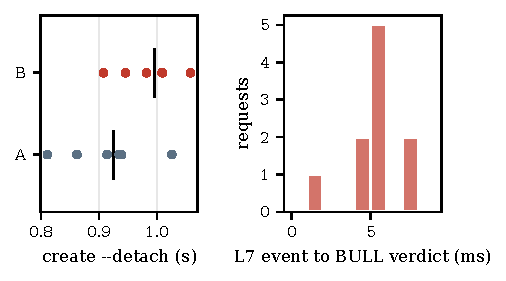
\includegraphics[width=\columnwidth]{figs/create_gap.pdf}
\caption{Left: sandbox admission time (bar = median). Right: interval from \openshell{}'s L7 event to \bull{}'s middleware verdict.}
\label{fig:create}
\end{figure}

\begin{table}[!t]
\caption{Latency Drift: Median of First vs.\ Last 50 Requests (ms)}
\label{tab:drift}
\centering
\small
\begin{tabular}{llrrr}
\toprule
\textbf{Metric} & \textbf{Phase} & \textbf{First 50} & \textbf{Last 50} & \textbf{Change} \\
\midrule
GET & A & 9.07 & 9.68 & +0.61 \\
GET & B & 14.89 & 17.67 & +2.77 \\
POST & A & 10.33 & 9.20 & -1.13 \\
POST & B & 19.49 & 25.13 & +5.64 \\
\bottomrule

\end{tabular}
\end{table}

Phase~B latency drifts upward within each loop (Fig.~\ref{fig:drift}, Table~\ref{tab:drift}): the GET median moved from \driftFirstGetB{} to \driftLastGetB{}\,ms and the POST median from \driftFirstPostB{} to \driftLastPostB{}\,ms, while Phase~A stayed near constant. \bull{}'s \texttt{AuditLedger} re-verifies the entire hash chain before each append, making append cost linear in ledger length; the ledger held \ledgerRecordsTotal{} records at the end of Phase~B. This is the most plausible cause but was not isolated experimentally. It also explains why POST overhead exceeds GET overhead: the POST loop ran second against a longer ledger.

%%% ------------------------------------------------------------------
\section{Findings About the Components}
%%% ------------------------------------------------------------------
\textbf{F1: \openshell{} L7 rules default to audit.} An endpoint with L7 rules and no \texttt{enforcement} field logs violations and forwards them; \openshell{} documents \texttt{audit} as the default~\cite{OS_Schema}. In C3b-A, a POST outside the only allowed path reached the destination, logged as \texttt{ALLOWED \ldots{} engine:l7}. \bull{} now refuses such policies at creation, replacement, and rule merge, accepting both the YAML form and the protobuf-JSON enum name \texttt{NETWORK\_ENFORCEMENT\_MODE\_ENFORCE}~\cite{PB_JSON}; \texttt{UNSPECIFIED} is treated as audit.

\textbf{F2: Transparent interception held.} Policy DNS resolved the destination to a trap address, so \texttt{curl --noproxy} traffic was still captured, L7-evaluated, and in Phase~B sent through \bull{}, which escalated it. Binary identity refused a Python client to an endpoint curl was allowed to use; a raw socket to a public address and UDP DNS both failed (C8).

\textbf{F3: Middleware metadata gaps in v0.1.2.} On the relay paths exercised, \openshell{} passes the literal scheme \texttt{https} to middleware for plaintext HTTP while its own OCSF events report \texttt{http}~\cite{OS_Relay}, and \texttt{RequestContext.originating\_process} is set to \texttt{None} for operator middleware~\cite{OS_MiddlewareSrc}, so \bull{} cannot bind a decision to the executable. \bull{} therefore does not trust \texttt{scheme}; the correlator compares host, port, and path only.

\textbf{F4: The extension contract is strict, and its failures closed.} A middleware reply whose \texttt{reason\_code} does not match \texttt{[a-z][a-z0-9\_]*} is treated as a middleware failure and the request is denied~\cite{OS_MiddlewareSrc}; an extension not declaring \texttt{openshell.<family>.contract} is refused at gateway start~\cite{OS_ExtProto}. Both mistakes appeared during integration and both stopped traffic rather than admitting it.

\textbf{F5: OCSF JSONL export requires a writable \texttt{/var/log} in the supervisor container}~\cite{OS_OCSFExport}, which the Docker driver's image did not provide; the same events were obtained through the gateway's log API.

\textbf{F6: \texttt{openshell sandbox exec} reads a non-TTY stdin to EOF before dispatching}~\cite{OS_CLIRun}; automation inheriting an open stdin blocks indefinitely.

%%% ------------------------------------------------------------------
\section{Defects Found in \bull{}}
%%% ------------------------------------------------------------------
Six defects passed \bull{}'s unit tests and surfaced only against the live gateway (Table~\ref{tab:defects}). Each has a regression test in \texttt{tests/test\_openshell\_authority.py}. Defect~3 is the most consequential: endpoints rendered as \texttt{host:40605.0} would never equal later \texttt{host:40605} comparisons, a latent source of false widening or missed widening.

\begin{table*}[!t]
\caption{Integration Defects Found and Fixed}
\label{tab:defects}
\centering
\scriptsize
\begin{tabularx}{\textwidth}{lYYY}
\toprule
\# & \textbf{Defect} & \textbf{Symptom against the live gateway} & \textbf{Fix} \\
\midrule
1 & Contract capabilities missing from \texttt{PeerMetadata} & Gateway refused to start & Declare \texttt{openshell.<family>.contract} as supported and required \\
2 & Dotted reason codes (\texttt{bull.denied}) & Every request denied as \texttt{response\_reason\_code\_invalid} (closed, but unusable) & Codes renamed \texttt{bull\_*}; grammar test \\
3 & Protobuf-JSON ports are doubles (\texttt{40605.0}) & Endpoint keys would not match later comparisons & Normalize to integers; cover every entry in \texttt{ports} \\
4 & No enforcement-mode check & \openshell{}-deny cases silently allowed (F1) & Refuse L7 rules not in \texttt{enforce} \\
5 & Enum form of enforcement not recognized & After fix 4, every sandbox refused & Accept \texttt{NETWORK\_ENFORCEMENT\_MODE\_ENFORCE} \\
6 & Correlator let a denied decision claim a nearby allowed receipt & C10 reported a false ``effect without allow'' & Assign receipts only to allowed decisions at or after decision time \\
\bottomrule
\end{tabularx}
\end{table*}

%%% ------------------------------------------------------------------
\section{Related Work and Positioning}
%%% ------------------------------------------------------------------
CaMeL separates control and data flow and applies capability policies to agent tool use~\cite{Debenedetti2025}; the provenance escalation here is a coarse, sandbox-granular instance of the same idea enforced at the network layer. gVisor and Firecracker isolate untrusted workloads with an application kernel or a lightweight VM~\cite{gVisor,Agache2020}; \openshell{} composes Landlock, seccomp, network namespaces, and an L7 proxy~\cite{OS_Repo,LinuxLandlock,LinuxSeccomp}. The contribution of this report is not a new isolation or authorization mechanism but a tested composition of the two through documented extension points, with destination-judged evidence and a joined audit trail.

%%% ------------------------------------------------------------------
\section{Limitations}
\label{sec:limits}
%%% ------------------------------------------------------------------
\textbf{Unauthenticated extension transport.} The middleware used plaintext gRPC with \texttt{allow\_insecure\_transport}, and \openshell{} warns that the service then cannot distinguish \openshell{} from any other network client. A bridge-local process could query \bull{} verdicts, although it could not alter an enforcement outcome. Production requires HTTPS with gateway-JWT validation; that configuration was not tested.

\textbf{Scope of mediation.} \bull{} sees HTTP egress and governed control-plane RPCs. It does not authorize process execution inside a sandbox; \openshell{}'s Landlock, seccomp, and binary identity contain exec. WebSocket sessions are not mediated. The ``exec'' half of the architecture's C7 is therefore \openshell{}'s guarantee, not \bull{}'s.

\textbf{Weak Phase~A evidence for C6.} The provider attachment was still awaiting the supervisor when the environment was inspected, so absence of the canary in Phase~A does not demonstrate \openshell{}'s placeholder mechanism. Phase~B's result rests on \bull{} refusing the attachment.

\textbf{Heuristic correlation.} OCSF shorthand carries no request identifier; the join uses sandbox, method, target, and time. It was exact here because requests were serialized; under concurrency, identical requests could swap row attribution without changing the counts on which C10 is judged. OCSF JSONL (F5) would remove this ambiguity.

\textbf{Single host, few runs.} One Docker host, no Kubernetes, VM, or hardware-isolated driver. Three complete runs were made; the first surfaced defect~5, and in the last two every case outcome was identical except C10, whose earlier failure was defect~6. Latency figures come from the final run and include shared-host noise. Approval latency (a human decision) is excluded.

%%% ------------------------------------------------------------------
\section{Conclusion}
%%% ------------------------------------------------------------------
On a live \openshell{} \osVersion{} gateway, \bull{} composed as a narrowing-only layer: every observed effect required both systems' consent; \bull{}'s absence failed closed on both data and control planes; provenance-based escalation stopped a post-read exfiltration that \openshell{}'s static policy permitted; unapproved widening and credential attachment were refused; and the two systems' records joined into one consistent trail. The measured cost was a median \deltaGet{}--\deltaPost{}\,ms per request in this build, much of it plausibly due to \bull{}'s linear-time ledger verification. The most consequential risk found was not in the composition but in a default: \openshell{}'s audit-mode L7 rules, which \bull{} now refuses.

\section*{Declarations}
\textbf{Research and authorship.} This manuscript describes the \bull{} project under Luis Minier / Anharmoniclabs. The author is a project stakeholder; the document is not an independent assessment. NVIDIA has not reviewed or endorsed this work; \openshell{} is cited as third-party software used under its Apache-2.0 license.

\textbf{AI assistance.} Claude Code (Anthropic) implemented the \openshell{} adapters, built \openshell{} from source, ran the experiment harness, and drafted this manuscript under the author's direction. AI-generated text is not experimental evidence; every measurement is generated from the recorded evidence files, whose SHA-256 digests are listed in Supplement~S6.

\textbf{Responsible reporting.} No secrets are published. The C6 canary credential was generated per run and verified absent from the evidence set; gateway JWT keys were generated per run and not retained.

\appendices

%%% ------------------------------------------------------------------
\section{Version and Evidence Identity}
%%% ------------------------------------------------------------------
\textbf{A1. \bull{}.} Repository \texttt{Anharmoniclabs/BULL}, branch \path{experiment/bull-openshell-20260928}, branched from \baseshort{}. The final experiment run executed \bull{} source identical to commit \expshort{}~\cite{BULL_Branch}.

\textbf{A2. \openshell{}.} \texttt{github.com/NVIDIA/OpenShell}, tag \texttt{v0.1.2}, commit \osshort{}~\cite{OS_Repo}. Middleware and interceptor stubs were generated from that tag's \texttt{.proto} files.

\textbf{A3. Evidence.} \path{docs/evidence/openshell-20260928/}~\cite{BULL_Evidence}; file digests in Supplement~S6.

\textbf{A4. Reproduction.}
{\footnotesize
\begin{verbatim}
cargo build --release \
  -p openshell-cli -p openshell-gateway \
  -p openshell-supervisor
cargo build --release \
  --target x86_64-unknown-linux-musl \
  -p openshell-sandbox
echo "172.17.0.1 host.openshell.internal" \
  >> /etc/hosts
python tools/openshell_experiment.py \
  --os-src $OS --latency-n 200 \
  --output \
  docs/evidence/openshell-20260928
python \
  tools/build_openshell_ieee_paper.py
\end{verbatim}}

%%% ------------------------------------------------------------------
\section{Claim-to-Evidence Ledger}
%%% ------------------------------------------------------------------
\begin{table*}[!t]
\caption{Claims, Supporting Evidence, and Boundaries of Interpretation}
\label{tab:ledger}
\centering
\small
\begin{tabularx}{\textwidth}{lYY}
\toprule
\textbf{Claim} & \textbf{Evidence} & \textbf{Not established} \\
\midrule
Effects required both systems' consent & C1--C3, C7; Table~\ref{tab:corr}; destination receipts (S3) & Behavior under concurrent or adversarially timed requests. \\
Escalation admits exactly once & C4 upstream count 1 with reuse refused & Approval UX or human-decision quality. \\
\bull{} absence fails closed & C9: POST denied, create refused; orphan event is a denial & Partial failures (slow, not dead, \bull{}); timeout tuning. \\
Unapproved widening refused & C5 new port, C5b ceiling, C3b audit mode & Widening through RPCs not bound by the interceptor. \\
Credential attachment governed & C6-B attach refused, canary absent & \openshell{} placeholder mechanism itself (C6-A inconclusive). \\
Native bypass contained & C8 OCSF evidence, EACCES, blocked UDP & Kernel or container-runtime escape. \\
Joined audit trail & \corrConsistent{}/\corrDecisions{} consistent, \corrUnexplained{} unexplained effects & Exact attribution under concurrency. \\
Overhead $\approx$\deltaGet--\deltaPost\,ms/request & Tables~\ref{tab:latency}, \ref{tab:stats}; raw samples S4 & Other hosts, authenticated transport, or an $O(1)$ ledger. \\
\bottomrule
\end{tabularx}
\end{table*}

\sloppy
\begin{thebibliography}{20}

\bibitem{OS_Repo}
NVIDIA, ``OpenShell,'' tag \texttt{v0.1.2}, commit \texttt{6648bd0}, 2026. [Online]. Available: \url{https://github.com/NVIDIA/OpenShell/tree/v0.1.2}

\bibitem{OS_MiddlewareDoc}
NVIDIA, ``Configure supervisor middleware,'' OpenShell documentation, \path{docs/extensibility/supervisor-middleware/configure.mdx}, v0.1.2. [Online]. Available: \url{https://github.com/NVIDIA/OpenShell/blob/v0.1.2/docs/extensibility/supervisor-middleware/configure.mdx}

\bibitem{OS_InterceptorDoc}
NVIDIA, ``Gateway interceptors,'' OpenShell documentation, \path{docs/extensibility/gateway-interceptors.mdx}, v0.1.2. [Online]. Available: \url{https://github.com/NVIDIA/OpenShell/blob/v0.1.2/docs/extensibility/gateway-interceptors.mdx}

\bibitem{OS_MiddlewareProto}
NVIDIA, ``Supervisor middleware protocol,'' \path{proto/supervisor_middleware.proto}, v0.1.2. [Online]. Available: \url{https://github.com/NVIDIA/OpenShell/blob/v0.1.2/proto/supervisor_middleware.proto}

\bibitem{OS_InterceptorProto}
NVIDIA, ``Gateway interceptor protocol,'' \path{proto/gateway_interceptor.proto}, v0.1.2. [Online]. Available: \url{https://github.com/NVIDIA/OpenShell/blob/v0.1.2/proto/gateway_interceptor.proto}

\bibitem{OS_Schema}
NVIDIA, ``Policy schema,'' OpenShell documentation, \path{docs/how-it-works/policies/schema.mdx}, v0.1.2. [Online]. Available: \url{https://github.com/NVIDIA/OpenShell/blob/v0.1.2/docs/how-it-works/policies/schema.mdx}

\bibitem{OS_Logging}
NVIDIA, ``Logging,'' OpenShell documentation, \path{docs/observability/logging.mdx}, v0.1.2. [Online]. Available: \url{https://github.com/NVIDIA/OpenShell/blob/v0.1.2/docs/observability/logging.mdx}

\bibitem{OS_OCSFExport}
NVIDIA, ``OCSF JSON export,'' OpenShell documentation, \path{docs/observability/ocsf-json-export.mdx}, v0.1.2. [Online]. Available: \url{https://github.com/NVIDIA/OpenShell/blob/v0.1.2/docs/observability/ocsf-json-export.mdx}

\bibitem{OS_MiddlewareSrc}
NVIDIA, ``Supervisor middleware runtime,'' \path{crates/openshell-supervisor-middleware/src/lib.rs} (reason-code grammar, line 824; \texttt{originating\_process}, line 1710), v0.1.2. [Online]. Available: \url{https://github.com/NVIDIA/OpenShell/blob/v0.1.2/crates/openshell-supervisor-middleware/src/lib.rs}

\bibitem{OS_Relay}
NVIDIA, ``L7 relay,'' \path{crates/openshell-supervisor-network/src/l7/relay.rs} (lines 1235, 1991), v0.1.2. [Online]. Available: \url{https://github.com/NVIDIA/OpenShell/blob/v0.1.2/crates/openshell-supervisor-network/src/l7/relay.rs}

\bibitem{OS_ExtProto}
NVIDIA, ``Extension protocol negotiation,'' \path{crates/openshell-core/src/extension_protocol.rs}, v0.1.2. [Online]. Available: \url{https://github.com/NVIDIA/OpenShell/blob/v0.1.2/crates/openshell-core/src/extension_protocol.rs}

\bibitem{OS_CLIRun}
NVIDIA, ``CLI sandbox exec,'' \path{crates/openshell-cli/src/run.rs} (line 1857), v0.1.2. [Online]. Available: \url{https://github.com/NVIDIA/OpenShell/blob/v0.1.2/crates/openshell-cli/src/run.rs}

\bibitem{RFC6902}
P.~Bryan and M.~Nottingham, ``JavaScript Object Notation (JSON) Patch,'' RFC~6902, IETF, 2013.

\bibitem{PB_JSON}
Google, ``ProtoJSON format,'' Protocol Buffers documentation. [Online]. Available: \url{https://protobuf.dev/programming-guides/json/}

\bibitem{BULL_Report}
L.~Minier, ``BULL: Blocking unauthorized logic loopholes,'' Anharmoniclabs technical report, v0.2, Sept. 20, 2026.

\bibitem{BULL_Branch}
Anharmoniclabs, ``BULL experiment branch \texttt{experiment/bull-openshell-20260928},'' 2026. [Online]. Available: \url{https://github.com/Anharmoniclabs/BULL/tree/experiment/bull-openshell-20260928}

\bibitem{BULL_Evidence}
Anharmoniclabs, ``BULL $\times$ OpenShell experiment evidence,'' \path{docs/evidence/openshell-20260928/}, 2026. [Online]. Available: \url{https://github.com/Anharmoniclabs/BULL/tree/experiment/bull-openshell-20260928/docs/evidence/openshell-20260928}

\bibitem{Debenedetti2025}
E.~Debenedetti \emph{et al.}, ``Defeating prompt injections by design,'' arXiv:2503.18813v2, 2025.

\bibitem{gVisor}
gVisor contributors, ``What is gVisor?'' [Online]. Available: \url{https://gvisor.dev/docs/}

\bibitem{Agache2020}
A.~Agache \emph{et al.}, ``Firecracker: Lightweight virtualization for serverless applications,'' in \emph{Proc. USENIX NSDI}, 2020.

\bibitem{LinuxSeccomp}
The Linux Kernel Documentation, ``Seccomp BPF (SECure COMPuting with filters).'' [Online]. Available: \url{https://docs.kernel.org/userspace-api/seccomp_filter.html}

\bibitem{LinuxLandlock}
The Linux Kernel Documentation, ``Landlock: unprivileged access control.'' [Online]. Available: \url{https://docs.kernel.org/userspace-api/landlock.html}

\end{thebibliography}

\section*{Biography}
\begingroup\footnotesize
\noindent\textbf{Luis Minier} is an independent researcher based in New York, NY, USA.\par
\endgroup

%%% ------------------------------------------------------------------
%%% Supplementary data: complete datasets, generated from the evidence
%%% ------------------------------------------------------------------
\onecolumn
\section*{Supplementary Material: Complete Datasets}
All tables below are generated verbatim from the evidence files listed in S6.

\subsection*{S1. Complete Case Results (\texttt{cases.csv})}
\scriptsize
\begin{longtable}{|p{0.3cm}|p{0.7cm}|p{2.6cm}|p{2.2cm}|p{8.0cm}|p{0.5cm}|}
\hline
\textbf{Ph.} & \textbf{Case} & \textbf{Property} & \textbf{Expected} & \textbf{Observed} & \textbf{Pass} \\ \hline
\endhead
A & setup & create coder & created & \texttt{\scriptsize ok} & yes \\ \hline
A & setup & create reader & created & \texttt{\scriptsize ok} & yes \\ \hline
A & C1 & BULL ALLOW + OpenShell ALLOW executes & reached upstream & \texttt{\scriptsize http 200; reached=\allowbreak{}True} & yes \\ \hline
A & C2 & BULL DENY + OpenShell ALLOW is blocked & reached (no BULL) & \texttt{\scriptsize http 200; reached=\allowbreak{}True} & yes \\ \hline
A & C3 & BULL ALLOW + OpenShell DENY is blocked & not reached & \texttt{\scriptsize http 403; reached=\allowbreak{}False} & yes \\ \hline
A & C3b & L7 rules in default audit mode (OpenShell only) & observe:\allowbreak{} violation allowed & \texttt{\scriptsize created=\allowbreak{}True; admin POST reached=\allowbreak{}True} & yes \\ \hline
A & C4 & Escalation without BULL & reached (no approval concept) & \texttt{\scriptsize http 200; reached=\allowbreak{}True} & yes \\ \hline
A & C7 & Internet-\allowbreak{}derived content -\allowbreak{}\textgreater{} POST without BULL & reached & \texttt{\scriptsize reached=\allowbreak{}True} & yes \\ \hline
A & C5 & Policy widening without BULL & applied & \texttt{\scriptsize ok Policy version 3 submitted (hash:\allowbreak{} de96f00b071a) ok Policy version 3 loaded (active version:\allowbreak{} 3)} & yes \\ \hline
A & C8 & Native tool bypass (no proxy,\allowbreak{} other binary,\allowbreak{} raw socket,\allowbreak{} DNS) contained & no unmediated effect; raw socket and DNS fail & \texttt{\scriptsize \{"noproxy\_\allowbreak{}direct":\allowbreak{} \{"rc":\allowbreak{} 0,\allowbreak{} "out":\allowbreak{} "\{\textbackslash{}"stored\textbackslash{}":\allowbreak{}true\}"\},\allowbreak{} "python\_\allowbreak{}socket":\allowbreak{} \{"rc":\allowbreak{} 1,\allowbreak{} "out":\allowbreak{} "raise exceptions[0]\textbackslash{}n File \textbackslash{}"/\allowbreak{}usr/\allowbreak{}lib/\allowbreak{}python3.\allowbreak{}12/\allowbreak{}socket.\allowbreak{}py\textbackslash{}",\allowbreak{} line 837,\allowbreak{} in create\_\allowbreak{}connection\textbackslash{}n sock.\allowbreak{}connect(sa)\textbackslash{}nPermissionError:\allowbreak{} [Errno 13] Permission denied"\},\allowbreak{} "python\_\allowbreak{}http":\allowbreak{} \{"rc":\allowbreak{} 1,\allowbreak{} "out":\allowbreak{} "File \textbackslash{}"/\allowbreak{}usr/\allowbreak{}lib/\allowbreak{}python3.\allowbreak{}12/\allowbreak{}urllib/\allowbreak{}request.\allowbreak{}py\textbackslash{}",\allowbreak{} line 1347,\allowbreak{} in do\_\allowbreak{}open\textbackslash{}n raise URLError(err)\textbackslash{}nurllib.\allowbreak{}error.\allowbreak{}URLError:\allowbreak{} \textless{}urlopen error [Errno 13] Permission denied\textgreater{}"\},\allowbreak{} "dns\_\allowbreak{}udp":\allowbreak{} \{"rc":\allowbreak{} 1,\allowbreak{} "out":\allowbreak{} "Traceback (most recent call last):\allowbreak{}\textbackslash{}n File \textbackslash{}"\textless{}string\textgreater{}\textbackslash{}",\allowbreak{} line 1,\allowbreak{} in \textless{}module\textgreater{}\textbackslash{}nOSError:\allowbreak{} [Errno 89] Destination address required"\},\allowbreak{} "/\allowbreak{}v1/\allowbreak{}x":\allowbreak{} \{"reached\_\allowbreak{}upstream":\allowbreak{} true,\allowbreak{} "ocsf\_\allowbreak{}engines":\allowbreak{} ["l7"]\},\allowbreak{} "/\allowbreak{}v1/\allowbreak{}y":\allowbreak{} \{"reached\_\allowbreak{}upstream":\allowbreak{} false,\allowbreak{} "ocsf\_\allowbreak{}engines":\allowbreak{} []\}\}} & yes \\ \hline
A & C6 & Provider credential not readable (OpenShell placeholder) & secret not in sandbox env & \texttt{\scriptsize provider\_\allowbreak{}created=\allowbreak{}True (ok Created provider canary); attach rc=\allowbreak{}0 coder /\allowbreak{} canary:\allowbreak{} persisted (waiting\_\allowbreak{}for\_\allowbreak{}supervisor) Receipt:\allowbreak{} 35fb08f6-\allowbreak{}612a-\allowbreak{}452f-\allowbreak{}8b36-\allowbreak{}c2987b4f427d Persisted:\allowbreak{} 2026-\allowbreak{}09-\allowbreak{}28T18:\allowbreak{}12:\allowbreak{}43.\allowbreak{}381635941Z; secret\_\allowbreak{}visible=\allowbreak{}False} & yes \\ \hline
A & C10 & Audit trail without BULL (OpenShell OCSF only) & observe:\allowbreak{} OCSF events,\allowbreak{} no authority decision record & \texttt{\scriptsize \{"ocsf\_\allowbreak{}http\_\allowbreak{}events":\allowbreak{} \{"l7":\allowbreak{} 8,\allowbreak{} "middleware":\allowbreak{} 0\},\allowbreak{} "upstream\_\allowbreak{}receipts":\allowbreak{} 7\}} & yes \\ \hline
B & setup & create coder & created & \texttt{\scriptsize ok} & yes \\ \hline
B & setup & create reader & created & \texttt{\scriptsize ok} & yes \\ \hline
B & C1 & BULL ALLOW + OpenShell ALLOW executes & reached upstream & \texttt{\scriptsize http 200; reached=\allowbreak{}True} & yes \\ \hline
B & C2 & BULL DENY + OpenShell ALLOW is blocked & not reached & \texttt{\scriptsize http 403; reached=\allowbreak{}False} & yes \\ \hline
B & C3 & BULL ALLOW + OpenShell DENY is blocked & not reached & \texttt{\scriptsize http 403; reached=\allowbreak{}False} & yes \\ \hline
B & C3b & L7 rules in default audit mode are refused at creation & create refused (bull\_\allowbreak{}l7\_\allowbreak{}audit\_\allowbreak{}mode) & \texttt{\scriptsize created=\allowbreak{}False; Error:\allowbreak{} x code:\allowbreak{} 'The caller does not have permission to execute the specified operation',\allowbreak{} message:\allowbreak{} "L7 rules must set enforcement:\allowbreak{} enforce:\allowbreak{} ['api:\allowbreak{}host.\allowbreak{}openshell.\allowbreak{}internal',\allowbreak{} 'docs:\allowbreak{}host.\allowbreak{}openshell.\allowbreak{}internal',\allowbreak{} 'news:\allowbreak{}host.\allowbreak{}openshell.\allowbreak{}internal']"} & yes \\ \hline
B & C4 & BULL ESCALATE:\allowbreak{} no effect before approval; exactly one after & 0 before,\allowbreak{} 1 after approval,\allowbreak{} 0 on reuse & \texttt{\scriptsize \{"first\_\allowbreak{}http":\allowbreak{} "403",\allowbreak{} "pending":\allowbreak{} 1,\allowbreak{} "approved":\allowbreak{} true,\allowbreak{} "retry\_\allowbreak{}http":\allowbreak{} "200",\allowbreak{} "third\_\allowbreak{}http":\allowbreak{} "403",\allowbreak{} "upstream\_\allowbreak{}count":\allowbreak{} 1\}} & yes \\ \hline
B & C7 & Internet-\allowbreak{}derived content -\allowbreak{}\textgreater{} POST hits BULL provenance control & escalated & \texttt{\scriptsize first attempt http 403,\allowbreak{} reached=\allowbreak{}False} & yes \\ \hline
B & C5 & Unauthorized policy widening rejected & rejected pending approval & \texttt{\scriptsize Error:\allowbreak{} x code:\allowbreak{} 'The caller does not have permission to execute the specified operation',\allowbreak{} message:\allowbreak{} "approval d029e1ad44e44632 required to widen policy with ['host.\allowbreak{}openshell.\allowbreak{}internal:\allowbreak{}9']"} & yes \\ \hline
B & C5b & Sandbox with host outside BULL ceiling refused & rejected & \texttt{\scriptsize Error:\allowbreak{} x code:\allowbreak{} 'The caller does not have permission to execute the specified operation',\allowbreak{} message:\allowbreak{} "policy grants hosts outside the signed BULL ceiling:\allowbreak{} ['attacker.\allowbreak{}example']"} & yes \\ \hline
B & C8 & Native tool bypass (no proxy,\allowbreak{} other binary,\allowbreak{} raw socket,\allowbreak{} DNS) contained & no unmediated effect; raw socket and DNS fail & \texttt{\scriptsize \{"noproxy\_\allowbreak{}direct":\allowbreak{} \{"rc":\allowbreak{} 0,\allowbreak{} "out":\allowbreak{} "enshell.\allowbreak{}internal\textbackslash{}",\allowbreak{}\textbackslash{}"layer\textbackslash{}":\allowbreak{}\textbackslash{}"l7\textbackslash{}",\allowbreak{}\textbackslash{}"method\textbackslash{}":\allowbreak{}\textbackslash{}"POST\textbackslash{}",\allowbreak{}\textbackslash{}"middleware\textbackslash{}":\allowbreak{}\textbackslash{}"bull-\allowbreak{}governance\textbackslash{}",\allowbreak{}\textbackslash{}"path\textbackslash{}":\allowbreak{}\textbackslash{}"/\allowbreak{}v1/\allowbreak{}x\textbackslash{}",\allowbreak{}\textbackslash{}"policy\textbackslash{}":\allowbreak{}\textbackslash{}"api\textbackslash{}",\allowbreak{}\textbackslash{}"port\textbackslash{}":\allowbreak{}35911,\allowbreak{}\textbackslash{}"reason\_\allowbreak{}code\textbackslash{}":\allowbreak{}\textbackslash{}"bull\_\allowbreak{}approval\_\allowbreak{}required\textbackslash{}"\}"\},\allowbreak{} "python\_\allowbreak{}socket":\allowbreak{} \{"rc":\allowbreak{} 1,\allowbreak{} "out":\allowbreak{} "raise exceptions[0]\textbackslash{}n File \textbackslash{}"/\allowbreak{}usr/\allowbreak{}lib/\allowbreak{}python3.\allowbreak{}12/\allowbreak{}socket.\allowbreak{}py\textbackslash{}",\allowbreak{} line 837,\allowbreak{} in create\_\allowbreak{}connection\textbackslash{}n sock.\allowbreak{}connect(sa)\textbackslash{}nPermissionError:\allowbreak{} [Errno 13] Permission denied"\},\allowbreak{} "python\_\allowbreak{}http":\allowbreak{} \{"rc":\allowbreak{} 1,\allowbreak{} "out":\allowbreak{} "File \textbackslash{}"/\allowbreak{}usr/\allowbreak{}lib/\allowbreak{}python3.\allowbreak{}12/\allowbreak{}urllib/\allowbreak{}request.\allowbreak{}py\textbackslash{}",\allowbreak{} line 1347,\allowbreak{} in do\_\allowbreak{}open\textbackslash{}n raise URLError(err)\textbackslash{}nurllib.\allowbreak{}error.\allowbreak{}URLError:\allowbreak{} \textless{}urlopen error [Errno 13] Permission denied\textgreater{}"\},\allowbreak{} "dns\_\allowbreak{}udp":\allowbreak{} \{"rc":\allowbreak{} 1,\allowbreak{} "out":\allowbreak{} "Traceback (most recent call last):\allowbreak{}\textbackslash{}n File \textbackslash{}"\textless{}string\textgreater{}\textbackslash{}",\allowbreak{} line 1,\allowbreak{} in \textless{}module\textgreater{}\textbackslash{}nOSError:\allowbreak{} [Errno 89] Destination address required"\},\allowbreak{} "/\allowbreak{}v1/\allowbreak{}x":\allowbreak{} \{"reached\_\allowbreak{}upstream":\allowbreak{} false,\allowbreak{} "ocsf\_\allowbreak{}engines":\allowbreak{} ["l7",\allowbreak{} "middleware"]\},\allowbreak{} "/\allowbreak{}v1/\allowbreak{}y":\allowbreak{} \{"reached\_\allowbreak{}upstream":\allowbreak{} false,\allowbreak{} "ocsf\_\allowbreak{}engines":\allowbreak{} []\}\}} & yes \\ \hline
B & C6 & Provider attach governed; credential never readable by the agent & attach refused (no credential.\allowbreak{}use grant); secret not in sandbox & \texttt{\scriptsize provider\_\allowbreak{}created=\allowbreak{}True (ok Created provider canary); attach:\allowbreak{} Error:\allowbreak{} x provider attachment failed (The caller does not have permission to execute the specified operation); secret\_\allowbreak{}visible=\allowbreak{}False} & yes \\ \hline
B & C9 & BULL unavailable -\allowbreak{}\textgreater{} egress and sandbox creation fail closed & not reached; create refused & \texttt{\scriptsize post http 403 reached=\allowbreak{}False; create\_\allowbreak{}while\_\allowbreak{}down=\allowbreak{}False; after\_\allowbreak{}restart\_\allowbreak{}docs\_\allowbreak{}http=\allowbreak{}200} & yes \\ \hline
B & C10 & OpenShell events + BULL decisions + effects correlate & every decision matched,\allowbreak{} consistent; no unexplained effect; ledger verifies & \texttt{\scriptsize \{"bull\_\allowbreak{}decisions":\allowbreak{} 9,\allowbreak{} "matched\_\allowbreak{}openshell\_\allowbreak{}event":\allowbreak{} 9,\allowbreak{} "consistent":\allowbreak{} 9,\allowbreak{} "effects\_\allowbreak{}without\_\allowbreak{}bull\_\allowbreak{}allow":\allowbreak{} 0,\allowbreak{} "openshell\_\allowbreak{}events\_\allowbreak{}without\_\allowbreak{}bull\_\allowbreak{}decision":\allowbreak{} 1,\allowbreak{} "orphans\_\allowbreak{}fail\_\allowbreak{}closed":\allowbreak{} true,\allowbreak{} "ledger\_\allowbreak{}valid":\allowbreak{} true,\allowbreak{} "ledger\_\allowbreak{}records":\allowbreak{} 19,\allowbreak{} "ocsf\_\allowbreak{}http\_\allowbreak{}events":\allowbreak{} \{"l7":\allowbreak{} 11,\allowbreak{} "middleware":\allowbreak{} 10\},\allowbreak{} "upstream\_\allowbreak{}receipts":\allowbreak{} 5\}} & yes \\ \hline

\end{longtable}

\normalsize
\subsection*{S2. Audit Join, Phase B (\texttt{correlation.json})}
\scriptsize
\setlength{\tabcolsep}{3pt}
\begin{longtable}{rllp{2.9cm}llp{1.9cm}p{2.4cm}llll}
\toprule
\# & \textbf{Sbx} & \textbf{Meth.} & \textbf{Resource} & \textbf{Prov.} & \textbf{\bull{}} & \textbf{Code} & \textbf{Approval} & \textbf{L7} & \textbf{MW} & \textbf{Eff.} & \textbf{Ledger} \\
\midrule
\endhead
1 & coder & GET & \texttt{host.\allowbreak{}openshell.\allowbreak{}internal:\allowbreak{}40959/\allowbreak{}guide} & local\_trusted & ALLOW & bull\_\allowbreak{}allowed & \texttt{} & ALLOWED & ALLOWED & yes & \texttt{f0fdd9b52d0c} \\
2 & coder & POST & \texttt{host.\allowbreak{}openshell.\allowbreak{}internal:\allowbreak{}35911/\allowbreak{}v1/\allowbreak{}records} & local\_trusted & ALLOW & bull\_\allowbreak{}allowed & \texttt{} & ALLOWED & ALLOWED & yes & \texttt{00c66c941d0d} \\
3 & reader & POST & \texttt{host.\allowbreak{}openshell.\allowbreak{}internal:\allowbreak{}35911/\allowbreak{}v1/\allowbreak{}records} & local\_trusted & DENY & bull\_\allowbreak{}denied & \texttt{} & ALLOWED & DENIED & no & \texttt{bfbdacde8424} \\
4 & coder & GET & \texttt{host.\allowbreak{}openshell.\allowbreak{}internal:\allowbreak{}46731/\allowbreak{}article} & local\_trusted & ALLOW & bull\_\allowbreak{}allowed & \texttt{} & ALLOWED & ALLOWED & yes & \texttt{f50244dca304} \\
5 & coder & POST & \texttt{host.\allowbreak{}openshell.\allowbreak{}internal:\allowbreak{}35911/\allowbreak{}v1/\allowbreak{}records} & internet & ESCALATE & bull\_\allowbreak{}approval\_\allowbreak{}required & \texttt{36b9cbbcf4819059} & ALLOWED & DENIED & no & \texttt{bb0324f51685} \\
6 & coder & POST & \texttt{host.\allowbreak{}openshell.\allowbreak{}internal:\allowbreak{}35911/\allowbreak{}v1/\allowbreak{}records} & internet & ESCALATE & bull\_\allowbreak{}approved & \texttt{36b9cbbcf4819059} & ALLOWED & ALLOWED & yes & \texttt{804e34a6b6c0} \\
7 & coder & POST & \texttt{host.\allowbreak{}openshell.\allowbreak{}internal:\allowbreak{}35911/\allowbreak{}v1/\allowbreak{}records} & internet & ESCALATE & bull\_\allowbreak{}approval\_\allowbreak{}required & \texttt{6452be302b3d2906} & ALLOWED & DENIED & no & \texttt{c9ef970549c5} \\
8 & coder & POST & \texttt{host.\allowbreak{}openshell.\allowbreak{}internal:\allowbreak{}35911/\allowbreak{}v1/\allowbreak{}x} & internet & ESCALATE & bull\_\allowbreak{}approval\_\allowbreak{}required & \texttt{fe51d8900f4821ec} & ALLOWED & DENIED & no & \texttt{8f9238c1744b} \\
9 & coder & GET & \texttt{host.\allowbreak{}openshell.\allowbreak{}internal:\allowbreak{}40959/\allowbreak{}after-\allowbreak{}restart} & internet & ALLOW & bull\_\allowbreak{}allowed & \texttt{} & ALLOWED & ALLOWED & yes & \texttt{82b54aba3d8d} \\
\bottomrule

\end{longtable}

\normalsize
\setlength{\tabcolsep}{6pt}
\subsection*{S3. \openshell{} OCSF HTTP Events and Destination Receipts}
\textbf{Phase A events} (\texttt{ocsf-*-A.txt}):
\scriptsize
\begin{longtable}{rlllp{0.8cm}p{4.6cm}p{4.8cm}}
\toprule
\textbf{Epoch (s)} & \textbf{Sandbox} & \textbf{Engine} & \textbf{Action} & \textbf{Meth.} & \textbf{Target} & \textbf{Reason} \\
\midrule
\endhead
1790619153.612 & coder & l7 & ALLOWED & GET & \texttt{host.\allowbreak{}openshell.\allowbreak{}internal:\allowbreak{}40959/\allowbreak{}guide} & \texttt{} \\
1790619153.667 & coder & l7 & ALLOWED & POST & \texttt{host.\allowbreak{}openshell.\allowbreak{}internal:\allowbreak{}35911/\allowbreak{}v1/\allowbreak{}records} & \texttt{} \\
1790619153.734 & reader & l7 & ALLOWED & POST & \texttt{host.\allowbreak{}openshell.\allowbreak{}internal:\allowbreak{}35911/\allowbreak{}v1/\allowbreak{}records} & \texttt{} \\
1790619153.793 & coder & l7 & DENIED & POST & \texttt{host.\allowbreak{}openshell.\allowbreak{}internal:\allowbreak{}35911/\allowbreak{}admin/\allowbreak{}delete} & \texttt{L7\_\allowbreak{}REQUEST deny POST host.\allowbreak{}openshell.\allowbreak{}internal:\allowbreak{}35911/\allowbreak{}admin/\allowbreak{}delete reason=\allowbreak{}POST /\allowbreak{}admin/\allowbreak{}delete not permitted by policy} \\
1790619154.773 & auditor & l7 & ALLOWED & POST & \texttt{host.\allowbreak{}openshell.\allowbreak{}internal:\allowbreak{}35911/\allowbreak{}admin/\allowbreak{}delete} & \texttt{} \\
1790619154.822 & coder & l7 & ALLOWED & GET & \texttt{host.\allowbreak{}openshell.\allowbreak{}internal:\allowbreak{}46731/\allowbreak{}article} & \texttt{} \\
1790619154.883 & coder & l7 & ALLOWED & POST & \texttt{host.\allowbreak{}openshell.\allowbreak{}internal:\allowbreak{}35911/\allowbreak{}v1/\allowbreak{}records} & \texttt{} \\
1790619162.980 & coder & l7 & ALLOWED & POST & \texttt{host.\allowbreak{}openshell.\allowbreak{}internal:\allowbreak{}35911/\allowbreak{}v1/\allowbreak{}x} & \texttt{} \\
\bottomrule

\end{longtable}
\normalsize
\textbf{Phase B events} (\texttt{ocsf-*-B.txt}):
\scriptsize
\begin{longtable}{rlllp{0.8cm}p{4.6cm}p{4.8cm}}
\toprule
\textbf{Epoch (s)} & \textbf{Sandbox} & \textbf{Engine} & \textbf{Action} & \textbf{Meth.} & \textbf{Target} & \textbf{Reason} \\
\midrule
\endhead
1790619184.386 & coder & l7 & ALLOWED & GET & \texttt{host.\allowbreak{}openshell.\allowbreak{}internal:\allowbreak{}40959/\allowbreak{}guide} & \texttt{} \\
1790619184.390 & coder & middleware & ALLOWED & GET & \texttt{host.\allowbreak{}openshell.\allowbreak{}internal:\allowbreak{}40959/\allowbreak{}guide} & \texttt{} \\
1790619184.437 & coder & l7 & ALLOWED & POST & \texttt{host.\allowbreak{}openshell.\allowbreak{}internal:\allowbreak{}35911/\allowbreak{}v1/\allowbreak{}records} & \texttt{} \\
1790619184.442 & coder & middleware & ALLOWED & POST & \texttt{host.\allowbreak{}openshell.\allowbreak{}internal:\allowbreak{}35911/\allowbreak{}v1/\allowbreak{}records} & \texttt{} \\
1790619184.504 & reader & l7 & ALLOWED & POST & \texttt{host.\allowbreak{}openshell.\allowbreak{}internal:\allowbreak{}35911/\allowbreak{}v1/\allowbreak{}records} & \texttt{} \\
1790619184.509 & reader & middleware & DENIED & POST & \texttt{host.\allowbreak{}openshell.\allowbreak{}internal:\allowbreak{}35911/\allowbreak{}v1/\allowbreak{}records} & \texttt{middleware\_\allowbreak{}denied:\allowbreak{}bull-\allowbreak{}governance:\allowbreak{}bull\_\allowbreak{}denied} \\
1790619184.567 & coder & l7 & DENIED & POST & \texttt{host.\allowbreak{}openshell.\allowbreak{}internal:\allowbreak{}35911/\allowbreak{}admin/\allowbreak{}delete} & \texttt{L7\_\allowbreak{}REQUEST deny POST host.\allowbreak{}openshell.\allowbreak{}internal:\allowbreak{}35911/\allowbreak{}admin/\allowbreak{}delete reason=\allowbreak{}POST /\allowbreak{}admin/\allowbreak{}delete not permitted by policy} \\
1790619184.645 & coder & l7 & ALLOWED & GET & \texttt{host.\allowbreak{}openshell.\allowbreak{}internal:\allowbreak{}46731/\allowbreak{}article} & \texttt{} \\
1790619184.649 & coder & middleware & ALLOWED & GET & \texttt{host.\allowbreak{}openshell.\allowbreak{}internal:\allowbreak{}46731/\allowbreak{}article} & \texttt{} \\
1790619184.704 & coder & l7 & ALLOWED & POST & \texttt{host.\allowbreak{}openshell.\allowbreak{}internal:\allowbreak{}35911/\allowbreak{}v1/\allowbreak{}records} & \texttt{} \\
1790619184.709 & coder & middleware & DENIED & POST & \texttt{host.\allowbreak{}openshell.\allowbreak{}internal:\allowbreak{}35911/\allowbreak{}v1/\allowbreak{}records} & \texttt{middleware\_\allowbreak{}denied:\allowbreak{}bull-\allowbreak{}governance:\allowbreak{}bull\_\allowbreak{}approval\_\allowbreak{}required} \\
1790619184.785 & coder & l7 & ALLOWED & POST & \texttt{host.\allowbreak{}openshell.\allowbreak{}internal:\allowbreak{}35911/\allowbreak{}v1/\allowbreak{}records} & \texttt{} \\
1790619184.790 & coder & middleware & ALLOWED & POST & \texttt{host.\allowbreak{}openshell.\allowbreak{}internal:\allowbreak{}35911/\allowbreak{}v1/\allowbreak{}records} & \texttt{} \\
1790619184.845 & coder & l7 & ALLOWED & POST & \texttt{host.\allowbreak{}openshell.\allowbreak{}internal:\allowbreak{}35911/\allowbreak{}v1/\allowbreak{}records} & \texttt{} \\
1790619184.852 & coder & middleware & DENIED & POST & \texttt{host.\allowbreak{}openshell.\allowbreak{}internal:\allowbreak{}35911/\allowbreak{}v1/\allowbreak{}records} & \texttt{middleware\_\allowbreak{}denied:\allowbreak{}bull-\allowbreak{}governance:\allowbreak{}bull\_\allowbreak{}approval\_\allowbreak{}required} \\
1790619184.957 & coder & l7 & ALLOWED & POST & \texttt{host.\allowbreak{}openshell.\allowbreak{}internal:\allowbreak{}35911/\allowbreak{}v1/\allowbreak{}x} & \texttt{} \\
1790619184.962 & coder & middleware & DENIED & POST & \texttt{host.\allowbreak{}openshell.\allowbreak{}internal:\allowbreak{}35911/\allowbreak{}v1/\allowbreak{}x} & \texttt{middleware\_\allowbreak{}denied:\allowbreak{}bull-\allowbreak{}governance:\allowbreak{}bull\_\allowbreak{}approval\_\allowbreak{}required} \\
1790619185.512 & coder & l7 & ALLOWED & POST & \texttt{host.\allowbreak{}openshell.\allowbreak{}internal:\allowbreak{}35911/\allowbreak{}v1/\allowbreak{}records} & \texttt{} \\
1790619185.513 & coder & middleware & DENIED & POST & \texttt{host.\allowbreak{}openshell.\allowbreak{}internal:\allowbreak{}35911/\allowbreak{}v1/\allowbreak{}records} & \texttt{middleware\_\allowbreak{}failed:\allowbreak{} external\_\allowbreak{}service\_\allowbreak{}error} \\
1790619185.877 & coder & l7 & ALLOWED & GET & \texttt{host.\allowbreak{}openshell.\allowbreak{}internal:\allowbreak{}40959/\allowbreak{}after-\allowbreak{}restart} & \texttt{} \\
1790619185.884 & coder & middleware & ALLOWED & GET & \texttt{host.\allowbreak{}openshell.\allowbreak{}internal:\allowbreak{}40959/\allowbreak{}after-\allowbreak{}restart} & \texttt{} \\
\bottomrule

\end{longtable}
\normalsize
\textbf{Destination receipts, Phase A} (\texttt{upstream-receipts-A.json}):
\scriptsize
\begin{longtable}{rlp{11cm}}
\toprule
\textbf{Epoch (s)} & \textbf{Method} & \textbf{URL} \\
\midrule
\endhead
1790619153.613 & GET & \texttt{http:\allowbreak{}/\allowbreak{}/\allowbreak{}host.\allowbreak{}openshell.\allowbreak{}internal:\allowbreak{}40959/\allowbreak{}guide} \\
1790619153.668 & POST & \texttt{http:\allowbreak{}/\allowbreak{}/\allowbreak{}host.\allowbreak{}openshell.\allowbreak{}internal:\allowbreak{}35911/\allowbreak{}v1/\allowbreak{}records} \\
1790619153.735 & POST & \texttt{http:\allowbreak{}/\allowbreak{}/\allowbreak{}host.\allowbreak{}openshell.\allowbreak{}internal:\allowbreak{}35911/\allowbreak{}v1/\allowbreak{}records} \\
1790619154.775 & POST & \texttt{http:\allowbreak{}/\allowbreak{}/\allowbreak{}host.\allowbreak{}openshell.\allowbreak{}internal:\allowbreak{}35911/\allowbreak{}admin/\allowbreak{}delete} \\
1790619154.827 & GET & \texttt{http:\allowbreak{}/\allowbreak{}/\allowbreak{}host.\allowbreak{}openshell.\allowbreak{}internal:\allowbreak{}46731/\allowbreak{}article} \\
1790619154.884 & POST & \texttt{http:\allowbreak{}/\allowbreak{}/\allowbreak{}host.\allowbreak{}openshell.\allowbreak{}internal:\allowbreak{}35911/\allowbreak{}v1/\allowbreak{}records} \\
1790619162.980 & POST & \texttt{http:\allowbreak{}/\allowbreak{}/\allowbreak{}host.\allowbreak{}openshell.\allowbreak{}internal:\allowbreak{}35911/\allowbreak{}v1/\allowbreak{}x} \\
\bottomrule

\end{longtable}
\normalsize
\textbf{Destination receipts, Phase B} (\texttt{upstream-receipts-B.json}):
\scriptsize
\begin{longtable}{rlp{11cm}}
\toprule
\textbf{Epoch (s)} & \textbf{Method} & \textbf{URL} \\
\midrule
\endhead
1790619184.391 & GET & \texttt{http:\allowbreak{}/\allowbreak{}/\allowbreak{}host.\allowbreak{}openshell.\allowbreak{}internal:\allowbreak{}40959/\allowbreak{}guide} \\
1790619184.443 & POST & \texttt{http:\allowbreak{}/\allowbreak{}/\allowbreak{}host.\allowbreak{}openshell.\allowbreak{}internal:\allowbreak{}35911/\allowbreak{}v1/\allowbreak{}records} \\
1790619184.650 & GET & \texttt{http:\allowbreak{}/\allowbreak{}/\allowbreak{}host.\allowbreak{}openshell.\allowbreak{}internal:\allowbreak{}46731/\allowbreak{}article} \\
1790619184.791 & POST & \texttt{http:\allowbreak{}/\allowbreak{}/\allowbreak{}host.\allowbreak{}openshell.\allowbreak{}internal:\allowbreak{}35911/\allowbreak{}v1/\allowbreak{}records} \\
1790619185.885 & GET & \texttt{http:\allowbreak{}/\allowbreak{}/\allowbreak{}host.\allowbreak{}openshell.\allowbreak{}internal:\allowbreak{}40959/\allowbreak{}after-\allowbreak{}restart} \\
\bottomrule

\end{longtable}

\normalsize
\subsection*{S4. Raw Request Latency, All Samples in Run Order (\texttt{latency-raw.json}, ms)}
\scriptsize
\begin{longtable}{r|rrrr||r|rrrr}
\toprule
\# & \textbf{A GET} & \textbf{B GET} & \textbf{A POST} & \textbf{B POST} & \# & \textbf{A GET} & \textbf{B GET} & \textbf{A POST} & \textbf{B POST} \\
\midrule
\endhead
1 & 18.761 & 28.393 & 8.973 & 22.982 & 101 & 8.071 & 17.330 & 9.711 & 17.383 \\
2 & 12.082 & 13.398 & 9.828 & 17.536 & 102 & 6.943 & 43.457 & 8.507 & 20.299 \\
3 & 9.509 & 16.153 & 10.169 & 16.234 & 103 & 7.253 & 27.507 & 8.778 & 20.679 \\
4 & 9.405 & 16.351 & 8.196 & 16.635 & 104 & 7.924 & 17.589 & 9.818 & 16.515 \\
5 & 8.891 & 21.402 & 9.279 & 20.731 & 105 & 7.589 & 19.970 & 8.505 & 24.811 \\
6 & 8.779 & 18.261 & 15.123 & 16.020 & 106 & 8.349 & 15.240 & 8.915 & 25.735 \\
7 & 11.115 & 13.653 & 17.178 & 20.223 & 107 & 9.731 & 15.225 & 8.958 & 34.712 \\
8 & 8.049 & 13.316 & 27.422 & 16.974 & 108 & 11.791 & 20.967 & 11.244 & 27.810 \\
9 & 13.269 & 15.529 & 20.176 & 19.716 & 109 & 7.049 & 15.038 & 11.374 & 23.515 \\
10 & 9.684 & 13.927 & 10.448 & 30.055 & 110 & 6.681 & 16.364 & 10.160 & 17.915 \\
11 & 10.325 & 17.886 & 10.835 & 21.414 & 111 & 7.226 & 17.535 & 13.773 & 20.919 \\
12 & 7.824 & 22.099 & 10.167 & 27.099 & 112 & 6.468 & 24.888 & 13.641 & 19.563 \\
13 & 16.403 & 25.889 & 10.569 & 19.259 & 113 & 7.792 & 26.118 & 25.978 & 21.430 \\
14 & 12.752 & 13.362 & 11.420 & 15.195 & 114 & 6.842 & 16.642 & 12.016 & 18.614 \\
15 & 23.452 & 14.859 & 9.379 & 19.972 & 115 & 8.497 & 22.623 & 9.829 & 22.709 \\
16 & 8.921 & 15.283 & 9.203 & 15.515 & 116 & 12.504 & 18.336 & 7.558 & 36.769 \\
17 & 10.346 & 13.993 & 10.329 & 17.309 & 117 & 10.670 & 18.693 & 10.093 & 17.720 \\
18 & 7.776 & 13.853 & 10.335 & 16.000 & 118 & 14.685 & 14.288 & 9.650 & 19.729 \\
19 & 8.739 & 12.642 & 10.983 & 21.327 & 119 & 7.340 & 15.888 & 9.443 & 22.476 \\
20 & 13.088 & 13.800 & 27.796 & 18.089 & 120 & 11.336 & 14.875 & 9.346 & 20.542 \\
21 & 7.811 & 16.106 & 9.571 & 24.082 & 121 & 9.917 & 17.019 & 12.103 & 18.229 \\
22 & 10.529 & 16.198 & 14.016 & 19.712 & 122 & 14.253 & 22.247 & 9.542 & 20.192 \\
23 & 8.137 & 13.453 & 12.275 & 15.761 & 123 & 11.214 & 20.949 & 10.281 & 21.025 \\
24 & 9.140 & 20.253 & 11.287 & 17.626 & 124 & 9.616 & 20.336 & 8.150 & 25.451 \\
25 & 12.208 & 19.172 & 7.755 & 16.371 & 125 & 10.614 & 20.399 & 8.504 & 29.375 \\
26 & 8.378 & 19.880 & 8.067 & 16.049 & 126 & 8.090 & 22.760 & 13.026 & 37.554 \\
27 & 8.335 & 19.921 & 7.070 & 18.806 & 127 & 9.512 & 16.609 & 10.924 & 20.262 \\
28 & 8.393 & 15.612 & 8.885 & 16.676 & 128 & 8.325 & 20.417 & 18.845 & 19.743 \\
29 & 10.935 & 15.972 & 10.640 & 18.229 & 129 & 8.863 & 17.001 & 15.106 & 18.652 \\
30 & 31.196 & 19.588 & 14.116 & 18.603 & 130 & 7.458 & 13.753 & 10.135 & 19.755 \\
31 & 8.365 & 14.231 & 11.323 & 15.776 & 131 & 9.051 & 19.030 & 7.042 & 22.145 \\
32 & 13.624 & 13.652 & 12.788 & 19.900 & 132 & 17.005 & 18.113 & 7.740 & 16.958 \\
33 & 8.235 & 13.891 & 8.191 & 29.976 & 133 & 14.545 & 25.585 & 7.114 & 25.112 \\
34 & 7.552 & 13.366 & 13.844 & 25.406 & 134 & 13.103 & 26.597 & 7.026 & 18.379 \\
35 & 7.609 & 14.925 & 11.756 & 20.492 & 135 & 8.218 & 20.523 & 6.645 & 29.107 \\
36 & 7.126 & 12.330 & 20.759 & 21.516 & 136 & 7.807 & 20.520 & 7.098 & 65.327 \\
37 & 9.323 & 11.430 & 25.899 & 16.308 & 137 & 8.961 & 20.623 & 9.421 & 32.676 \\
38 & 8.066 & 17.769 & 11.603 & 14.422 & 138 & 11.121 & 15.479 & 12.054 & 26.971 \\
39 & 10.471 & 20.163 & 11.027 & 18.334 & 139 & 9.871 & 17.658 & 9.773 & 25.423 \\
40 & 9.009 & 17.898 & 7.586 & 20.783 & 140 & 8.438 & 15.289 & 10.440 & 23.896 \\
41 & 8.558 & 14.865 & 6.908 & 22.535 & 141 & 11.215 & 16.656 & 8.841 & 17.635 \\
42 & 10.346 & 14.259 & 14.448 & 21.211 & 142 & 8.091 & 21.610 & 9.020 & 19.197 \\
43 & 8.698 & 18.774 & 7.712 & 28.948 & 143 & 13.692 & 20.467 & 8.675 & 25.504 \\
44 & 15.492 & 15.142 & 7.259 & 30.882 & 144 & 8.121 & 20.330 & 10.846 & 20.549 \\
45 & 7.458 & 13.890 & 8.557 & 26.767 & 145 & 8.693 & 24.268 & 21.169 & 26.329 \\
46 & 16.496 & 13.207 & 7.157 & 23.907 & 146 & 8.494 & 30.677 & 22.363 & 28.185 \\
47 & 16.190 & 12.685 & 8.424 & 20.139 & 147 & 9.828 & 26.029 & 10.469 & 28.169 \\
48 & 7.881 & 13.455 & 9.462 & 15.118 & 148 & 12.116 & 19.061 & 9.241 & 20.882 \\
49 & 8.497 & 13.960 & 9.843 & 27.652 & 149 & 20.079 & 19.759 & 7.436 & 21.861 \\
50 & 7.175 & 13.654 & 8.224 & 18.619 & 150 & 11.130 & 17.533 & 10.500 & 17.524 \\
51 & 6.823 & 21.881 & 12.149 & 20.690 & 151 & 8.513 & 16.252 & 7.457 & 18.400 \\
52 & 6.583 & 22.633 & 16.906 & 35.993 & 152 & 9.151 & 16.823 & 11.326 & 22.890 \\
53 & 6.359 & 15.158 & 15.633 & 28.010 & 153 & 8.381 & 15.994 & 9.706 & 26.394 \\
54 & 6.966 & 15.884 & 13.855 & 22.119 & 154 & 8.388 & 18.002 & 13.209 & 28.886 \\
55 & 6.897 & 15.306 & 10.556 & 21.346 & 155 & 11.850 & 17.657 & 11.032 & 28.153 \\
56 & 6.732 & 13.706 & 7.740 & 14.830 & 156 & 11.451 & 17.459 & 7.287 & 29.185 \\
57 & 8.383 & 12.483 & 9.161 & 16.623 & 157 & 7.988 & 26.985 & 9.482 & 26.337 \\
58 & 10.230 & 12.759 & 7.053 & 17.064 & 158 & 7.639 & 20.177 & 7.413 & 19.426 \\
59 & 8.336 & 11.845 & 8.959 & 17.768 & 159 & 7.564 & 19.360 & 7.582 & 18.346 \\
60 & 8.382 & 12.293 & 8.005 & 17.006 & 160 & 8.471 & 15.288 & 19.453 & 21.920 \\
61 & 8.036 & 13.138 & 7.365 & 14.476 & 161 & 8.723 & 17.825 & 11.950 & 20.278 \\
62 & 7.495 & 12.373 & 9.501 & 18.765 & 162 & 8.909 & 16.225 & 18.730 & 24.008 \\
63 & 10.908 & 18.720 & 15.446 & 21.850 & 163 & 10.005 & 14.169 & 8.570 & 19.676 \\
64 & 11.118 & 19.909 & 24.221 & 40.497 & 164 & 9.490 & 14.315 & 9.196 & 32.797 \\
65 & 9.298 & 24.941 & 13.106 & 18.139 & 165 & 11.326 & 14.366 & 8.901 & 26.548 \\
66 & 9.606 & 19.579 & 12.276 & 19.980 & 166 & 12.871 & 22.275 & 8.736 & 24.332 \\
67 & 10.025 & 19.171 & 17.220 & 16.153 & 167 & 10.502 & 21.282 & 9.533 & 23.036 \\
68 & 7.708 & 14.775 & 12.482 & 16.229 & 168 & 8.095 & 23.506 & 9.894 & 25.064 \\
69 & 7.405 & 13.444 & 19.582 & 16.137 & 169 & 7.385 & 20.225 & 7.770 & 26.089 \\
70 & 7.681 & 14.092 & 17.862 & 18.762 & 170 & 7.116 & 19.980 & 7.092 & 19.509 \\
71 & 8.181 & 14.331 & 8.999 & 16.922 & 171 & 8.575 & 16.198 & 10.458 & 18.261 \\
72 & 6.396 & 14.197 & 10.379 & 16.094 & 172 & 9.085 & 17.118 & 7.042 & 34.170 \\
73 & 8.128 & 14.365 & 9.689 & 21.216 & 173 & 13.911 & 17.859 & 7.297 & 54.996 \\
74 & 8.061 & 13.667 & 10.118 & 22.156 & 174 & 8.132 & 14.874 & 7.630 & 20.438 \\
75 & 7.120 & 13.519 & 9.125 & 27.987 & 175 & 13.108 & 15.021 & 7.679 & 21.329 \\
76 & 11.115 & 17.350 & 9.606 & 28.316 & 176 & 8.413 & 16.825 & 6.765 & 21.003 \\
77 & 7.356 & 22.122 & 8.946 & 18.191 & 177 & 9.282 & 15.678 & 13.433 & 25.784 \\
78 & 7.745 & 20.543 & 9.429 & 23.746 & 178 & 7.923 & 23.702 & 13.665 & 25.384 \\
79 & 7.944 & 19.535 & 7.856 & 20.253 & 179 & 13.546 & 32.220 & 20.082 & 17.963 \\
80 & 13.767 & 17.324 & 16.861 & 20.557 & 180 & 11.853 & 21.489 & 15.195 & 25.601 \\
81 & 7.838 & 16.620 & 11.333 & 21.830 & 181 & 17.836 & 20.372 & 7.894 & 37.606 \\
82 & 16.916 & 15.242 & 14.477 & 19.825 & 182 & 16.940 & 16.471 & 7.681 & 29.374 \\
83 & 15.090 & 15.592 & 10.820 & 17.941 & 183 & 7.790 & 16.152 & 7.764 & 33.889 \\
84 & 10.542 & 17.801 & 22.191 & 27.223 & 184 & 10.549 & 14.339 & 9.848 & 23.167 \\
85 & 8.770 & 17.586 & 12.048 & 20.390 & 185 & 9.878 & 15.723 & 9.077 & 26.266 \\
86 & 10.895 & 14.006 & 11.372 & 21.557 & 186 & 15.538 & 14.138 & 17.198 & 28.500 \\
87 & 8.112 & 12.416 & 9.138 & 20.557 & 187 & 12.587 & 19.041 & 7.772 & 20.875 \\
88 & 7.309 & 15.695 & 8.885 & 16.130 & 188 & 9.299 & 18.724 & 8.839 & 28.133 \\
89 & 8.175 & 18.425 & 17.580 & 17.707 & 189 & 7.095 & 22.936 & 8.567 & 31.442 \\
90 & 10.809 & 17.302 & 9.822 & 17.040 & 190 & 12.226 & 25.781 & 8.766 & 32.215 \\
91 & 8.637 & 21.284 & 9.967 & 16.369 & 191 & 14.394 & 20.135 & 10.899 & 21.311 \\
92 & 14.036 & 18.601 & 8.776 & 17.771 & 192 & 9.380 & 20.444 & 7.662 & 23.127 \\
93 & 7.269 & 15.815 & 9.631 & 18.958 & 193 & 12.771 & 16.938 & 25.801 & 26.049 \\
94 & 8.542 & 17.898 & 13.989 & 18.165 & 194 & 23.381 & 21.944 & 19.047 & 20.329 \\
95 & 8.114 & 15.616 & 18.521 & 17.790 & 195 & 12.467 & 16.960 & 21.662 & 25.188 \\
96 & 9.433 & 15.634 & 14.727 & 21.731 & 196 & 11.961 & 17.676 & 9.211 & 26.643 \\
97 & 10.372 & 14.632 & 10.972 & 39.468 & 197 & 12.553 & 17.142 & 10.449 & 24.594 \\
98 & 19.423 & 17.883 & 8.511 & 29.163 & 198 & 8.573 & 17.640 & 11.746 & 39.690 \\
99 & 14.908 & 13.316 & 33.856 & 22.711 & 199 & 12.377 & 27.050 & 11.336 & 18.292 \\
100 & 21.481 & 15.140 & 9.845 & 18.540 & 200 & 10.308 & 30.317 & 9.099 & 18.214 \\
\bottomrule

\end{longtable}

\normalsize
\subsection*{S5. Sandbox Creation Samples (s) and L7-to-Verdict Intervals (ms)}
\begin{center}
\small
\begin{tabular}{rrr}
\toprule
\# & \textbf{A} & \textbf{B} \\
\midrule
1 & 1.026 & 1.010 \\
2 & 0.935 & 0.908 \\
3 & 0.939 & 1.009 \\
4 & 0.914 & 0.946 \\
5 & 0.862 & 1.058 \\
6 & 0.811 & 0.982 \\
\bottomrule

\end{tabular}
\end{center}
L7-to-verdict intervals, Phase B, in event order: 4, 5, 4, 5, 5, 7, 5, 1, 7, 5


\subsection*{S6. Evidence File Integrity (SHA-256)}
Every number in this paper was computed from these files by \texttt{tools/build\_openshell\_ieee\_paper.py}.
\scriptsize
\begin{longtable}{lrl}
\toprule
\textbf{File} & \textbf{Bytes} & \textbf{SHA-256} \\
\midrule
\endhead
\texttt{README.md} & 1396 & \texttt{\scriptsize d4e8adae9887f56edb225a7d8114171c71bbc66671dfc924fe7f3bad65390218} \\
\texttt{bull-audit.jsonl} & 312291 & \texttt{\scriptsize 340a7cc304af900367c1ea221979cb81eab7f7808d4009f0ac067560669bd242} \\
\texttt{bull.log} & 52745 & \texttt{\scriptsize 8a1cbc68fd43d3cb92a416856a0f6b5fe1e9b4347402bb32ef383b0ed3bdeda7} \\
\texttt{cases.csv} & 6404 & \texttt{\scriptsize 23c4de9120031d4943246a07991e2f76b80a23c654049508d7df6d69101ff3d3} \\
\texttt{correlation.json} & 6496 & \texttt{\scriptsize c718ac4013c8a417fad372a432c0ee43c2df65e53989910653c1c1a608a4d666} \\
\texttt{gateway-A.log} & 242308 & \texttt{\scriptsize 9e8d586e4db5ea8a3347e92b487c0454162f2e92f76261c0a214a925b7659a0b} \\
\texttt{gateway-A.toml} & 496 & \texttt{\scriptsize 6ffdc55cfc57e629cd0a6e64f36115b2a15866d949e34ad9d94f6788b6d88f3c} \\
\texttt{gateway-B.log} & 261142 & \texttt{\scriptsize 93b8de8ab71267cd32867087d7ee2430d1e5957a09ad3a78587224ce4b02621d} \\
\texttt{gateway-B.toml} & 1628 & \texttt{\scriptsize fcc36360b7265a4c24b77f5def645cb51e3822774da0f68e3ef020ad96d79398} \\
\texttt{latency-raw.json} & 6662 & \texttt{\scriptsize f3c7d17932a1c567d9ad2003c1b356cf0917cfc0a8ddcd045746094fdd77f56c} \\
\texttt{latency.csv} & 503 & \texttt{\scriptsize 8c20b41183132722be2dbdb08bd0e840bb31392b616767ae200653d5ea04dac5} \\
\texttt{ocsf-auditor-A.txt} & 3463 & \texttt{\scriptsize 4aa278f9af100986efa226cc29f019e7b8ed119f2d27758ee4b8010e0e371d22} \\
\texttt{ocsf-auditor-B.txt} & 0 & \texttt{\scriptsize e3b0c44298fc1c149afbf4c8996fb92427ae41e4649b934ca495991b7852b855} \\
\texttt{ocsf-coder-A.txt} & 11799 & \texttt{\scriptsize 69ac92422596e1c0123b11929a4bd077d405695cd2e3aff847b5185820703d43} \\
\texttt{ocsf-coder-B.txt} & 15885 & \texttt{\scriptsize 990e98f0521ebfd1a4d30b4ff2791644d9e20d4bf6cd53461061da92ff194e1f} \\
\texttt{ocsf-reader-A.txt} & 3458 & \texttt{\scriptsize 48e6de30cece45547ca46bdddc46f072db52d3ac4ab2bc3713c4f9f847c7a6e6} \\
\texttt{ocsf-reader-B.txt} & 3148 & \texttt{\scriptsize 8f6c8810952f285096b751e1c44edd2009f1653663805a81ab9c9835c362d35b} \\
\texttt{policy.yaml} & 977 & \texttt{\scriptsize c77976ada5d58555020934678b4fbe05f2061301ef82851c5130e3bdaf7053c7} \\
\texttt{results.json} & 17122 & \texttt{\scriptsize 51e0f0c49c85cb296f93af6abdd4836b15c2bb54ce37d4485e24964531c81358} \\
\texttt{upstream-receipts-A.json} & 798 & \texttt{\scriptsize 51db4130544dfb67d84530bbfb4f177bc89e8451f1f18cf316d9f1e88961648f} \\
\texttt{upstream-receipts-B.json} & 574 & \texttt{\scriptsize fdbe5c9ef8862eda1fae1093302b6aafabbe135334a5170eb853ff4f431158df} \\
\bottomrule

\end{longtable}

\end{document}
